\documentclass[a4paper]{article}
\usepackage{cmap}
\usepackage[utf8]{inputenc}
\usepackage[T2A]{fontenc}
\usepackage[english,russian]{babel} 
\usepackage[left=15mm, top=15mm, right=15mm, bottom=42mm, nohead, nofoot]{geometry}
\usepackage{blindtext}  % рыба-текст
\usepackage{graphicx}  % изобржаения
\usepackage{float} % плавающие объекты
\usepackage{wrapfig}  % изобржаения
\usepackage{tikz} % графика
\usepackage{xcolor} % определение цветов
\usepackage{nicefrac} % красивые дроби
\usepackage{cancel} % сокращение
\usepackage{amsmath,amsfonts,amssymb} % математический пакет
\usepackage{hyperref}  % гиперссылки
\usepackage{fancybox,fancyhdr} % хедер и футер
\usepackage{listings} % код
\pagestyle{fancy}
\fancyhf{}
\fancyhead[L]{Лабораторная работа №2}
\fancyhead[R]{\textit{Преобразование Фурье}}
\fancyfoot[C]{\thepage}
\headsep=8mm
\footskip=20mm

\definecolor{urlcolor}{HTML}{3454D1}
\definecolor{linkcolor}{HTML}{3454D1}
\hypersetup{pdfstartview=FitH, linkcolor=linkcolor, urlcolor=urlcolor, colorlinks=true}

\definecolor{strings}{rgb}{0,0.6,0}
\definecolor{comments}{rgb}{0,0.3,0}
\definecolor{numbers}{rgb}{0.5,0.5,0.5}
\definecolor{keywords}{rgb}{0.09,0.61,0.95}
\definecolor{background}{rgb}{0.97,0.97,0.97}
\lstdefinestyle{codestyle}{
    backgroundcolor=\color{background},
    commentstyle=\color{comments},
    keywordstyle=\color{keywords},
    stringstyle=\color{strings},
    numberstyle=\tiny\color{numbers},
    basicstyle=\ttfamily\footnotesize,
    breakatwhitespace=false,
    breaklines=true,
    captionpos=b,
    inputencoding=utf8,
    keepspaces=true,
    numbers=left,
    numbersep=5pt,
    showspaces=false,
    showstringspaces=false,
    showtabs=false,
    tabsize=2,
    extendedchars=true,
    literate=
    {а}{{\cyra}}1
    {б}{{\cyrb}}1
    {в}{{\cyrv}}1
    {г}{{\cyrg}}1
    {д}{{\cyrd}}1
    {е}{{\cyre}}1
    {ж}{{\cyrzh}}1
    {з}{{\cyrz}}1
    {и}{{\cyri}}1
    {й}{{\cyrishrt}}1
    {к}{{\cyrk}}1
    {л}{{\cyrl}}1
    {м}{{\cyrm}}1
    {н}{{\cyrn}}1
    {о}{{\cyro}}1
    {п}{{\cyrp}}1
    {р}{{\cyrr}}1
    {с}{{\cyrs}}1
    {т}{{\cyrt}}1
    {у}{{\cyru}}1
    {ф}{{\cyrf}}1
    {х}{{\cyrh}}1
    {ц}{{\cyrc}}1
    {ч}{{\cyrch}}1
    {ш}{{\cyrsh}}1
    {щ}{{\cyrshch}}1
    {ъ}{{\cyrhrdsn}}1
    {ы}{{\cyrery}}1
    {ь}{{\cyrsftsn}}1
    {э}{{\cyrerev}}1
    {ю}{{\cyryu}}1
    {я}{{\cyrya}}1
    {А}{{\CYRA}}1
    {Б}{{\CYRB}}1
    {В}{{\CYRV}}1
    {Г}{{\CYRG}}1
    {Д}{{\CYR96}}1
    {Е}{{\CYRE}}1
    {Ж}{{\CYRZH}}1
    {З}{{\CYRZ}}1
    {И}{{\CYRI}}1
    {Й}{{\CYRISHRT}}1
    {К}{{\CYRK}}1
    {Л}{{\CYRL}}1
    {М}{{\CYRM}}1
    {Н}{{\CYRN}}1
    {О}{{\CYRO}}1
    {П}{{\CYRP}}1
    {Р}{{\CYRR}}1
    {С}{{\CYRS}}1
    {Т}{{\CYRT}}1
    {У}{{\CYRU}}1
    {Ф}{{\CYRF}}1
    {Х}{{\CYRH}}1
    {Ц}{{\CYRC}}1
    {Ч}{{\CYRCH}}1
    {Ш}{{\CYRSH}}1
    {Щ}{{\CYRSHCH}}1
    {Ъ}{{\CYRHRDSN}}1
    {Ы}{{\CYRERY}}1
    {Ь}{{\CYRSFTSN}}1
    {Э}{{\CYREREV}}1
    {Ю}{{\CYRYU}}1
    {Я}{{\CYRYA}}1
}

\lstset{style=codestyle}

\addto\captionsrussian{
  \renewcommand{\contentsname}
    {\centering Содержание}
}
\newcommand{\section}[1]{
    \phantomsection
    \addcontentsline{toc}{section}{#1}
    \section*{\centering #1}
}
\newcommand{\subsection}[1]{
    \phantomsection
    \addcontentsline{toc}{subsection}{#1}
    \subsection*{\centering #1}
}
\newcommand{\subsubsection}[1]{
    \phantomsection
    \addcontentsline{toc}{subsubsection}{#1}
    \subsubsection*{\centering #1}
}

\newlength{\tempheight}
\newcommand{\Let}{
\mathbin{\text{\settoheight{\tempheight}{\mathstrut}\raisebox{0.4\pgflinewidth}{
\tikz[baseline=0.5ex,line cap=round,line join=round] \draw (0,0) --++ (0.3em,0) --++ (0,2.3ex) --++ (-0.3em,0);
}}}}
\newcommand*\squared[1]{\tikz[baseline=(char.base)]{
            \node[shape=rectangle,draw,inner sep=4pt] (char) {#1};}}
\newcommand*\msquared[1]{\tikz[baseline=(char.base)]{
            \node[shape=rectangle,draw,inner sep=4pt] (char) {$\displaystyle #1$};}}
\newcommand{\at}{\biggr\rvert}
\newcommand{\shiftright}[3]{\makebox[#2][r]{\makebox[#1][l]{#3}}}
\newcommand{\e}{\;\text{e}}
\let\oldint\int
\def\int{\oldint\limits}
\DeclareRobustCommand{\divby}{%
  \mathrel{\vbox{\baselineskip.65ex\lineskiplimit0pt\hbox{.}\hbox{.}\hbox{.}}}%
}

\newcommand\NB{\textbf{N\kern-0.32em\textcolor{red}{B}}}

\begin{document}

\begin{titlepage}
    \begin{center}
        Федеральное государственное автономное образовательное \\ учреждение высшего образования \\[6pt]
        САНКТ-ПЕТЕРБУРГСКИЙ НАЦИОНАЛЬНЫЙ \\ ИССЛЕДОВАТЕЛЬСКИЙ УНИВЕРСИТЕТ ИТМО \\[16pt]
        Факультет систем управления и робототехники \\[26em]
        Лабораторная работа №2 \\[0.5em]
        \textbf{ПРЕОБРАЗОВАНИЕ ФУРЬЕ}
    \end{center}\,\\[10em]
    \begin{flushright}
        Студент: Заводин Е.Ю.\\
        Поток: ЧастМет R23 1.6 \\[0.5em]
        Преподаватели: Перегудин А.А.\\
        Догадин Е.В.
    \end{flushright}\,\\[6em]
    \begin{center}
        {\small Санкт-Петербург \\ 2025}
    \end{center}
\end{titlepage}
\setcounter{page}{2}
\tableofcontents\newpage

В первых двух заданиях используется унитарное преобразование Фурье к угловой частоте $\omega$:

$$\hat{f}(\omega) = \frac{1}{\sqrt{2\pi}}\int_{-\infty}^{\infty}f(t)\e^{-i\omega t}\,dt$$\

А также обратное преобразование
$$f(t) = \frac{1}{\sqrt{2\pi}}\int_{-\infty}^{\infty}\hat{f}(\omega)\e^{i\omega t}\,d\omega$$

\section{Вещественное задание}\

Зададим следующие три набора значений параметров $a, b: (1, 2), (2, 3), (1, 1)$ для дальнейшего построения графиков функций и соответствующих им Фурье-образов.

\subsection{Прямоугольная функция}\

Первая функция выглядит следующим образом:

$$
f(t) = \begin{cases}
    a, & \left| t \right| \in b \\
    0, & \left| t \right| > b
\end{cases}
$$\

Найдём её Фурье-образ. Нет смысла рассматривать интеграл за пределами отрезка $t \in [-b, b]$, так как там функция равна нулю. Перейти от разницы комплексных экспонент к синусу же помогает формула Эйлера:

$$
\hat{f}(\omega)=\frac{1}{\sqrt{2\pi}}\int_{-b}^{b}a\e^{-i\omega t}dt = \frac{a\e^{i\omega t}}{-\sqrt{2\pi}i\omega}\at^b_{-b} = \frac{a\left( \e^{i\omega b} - \e^{-i\omega b} \right)}{\omega i\sqrt{2\pi}} = \frac{2a\sin{\omega b}}{\omega\sqrt{2\pi}} = \frac{2ab}{\sqrt{2\pi}}\mathrm{sinc}\,\omega b
$$\

Перейдём к визуализации:

\begin{figure}[H]
    \begin{minipage}{0.5\textwidth}
        \centering 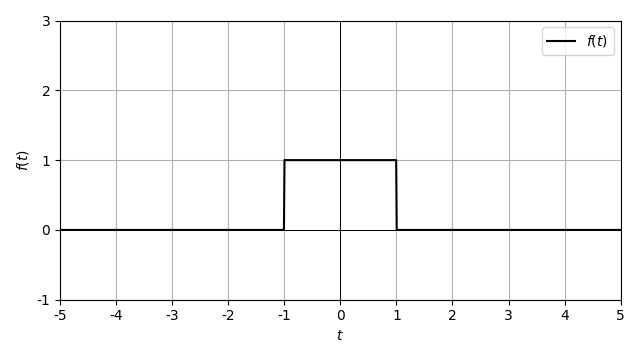
\includegraphics[width=\textwidth]{rectangular/real_graph_1_1.png}
        \caption{Прямоугольная функция, $a = 1, b = 1$}
    \end{minipage}\hfill
    \begin{minipage}{0.5\textwidth}
        \centering 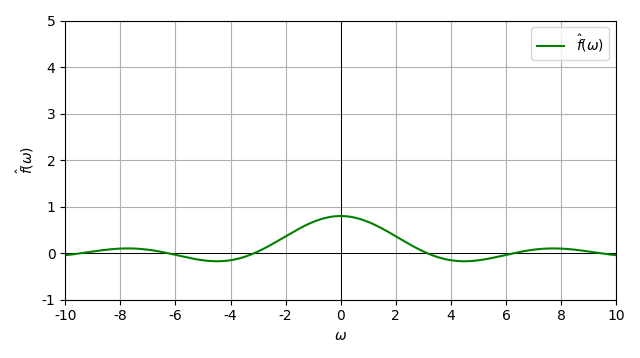
\includegraphics[width=\textwidth]{rectangular/real_fourier_1_1.png}
        \caption{Фурье-образ прямоугольной ф-ии, $a = 1, b = 1$}
    \end{minipage}\\[1em]
\end{figure}\noindent\

\begin{figure}[H]
        \begin{minipage}{0.5\textwidth}
        \centering 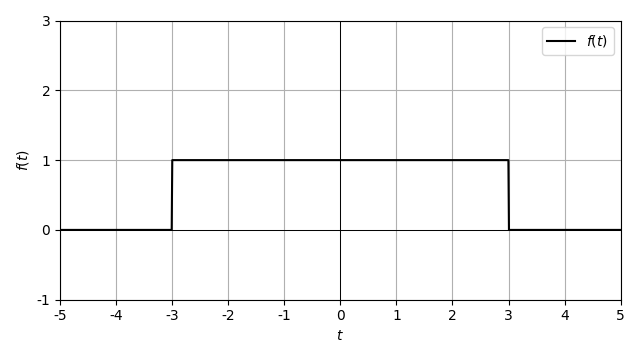
\includegraphics[width=\textwidth]{rectangular/real_graph_1_3.png}
        \caption{Прямоугольная функция, $a = 1, b = 3$}
    \end{minipage}\hfill
    \begin{minipage}{0.5\textwidth}
        \centering 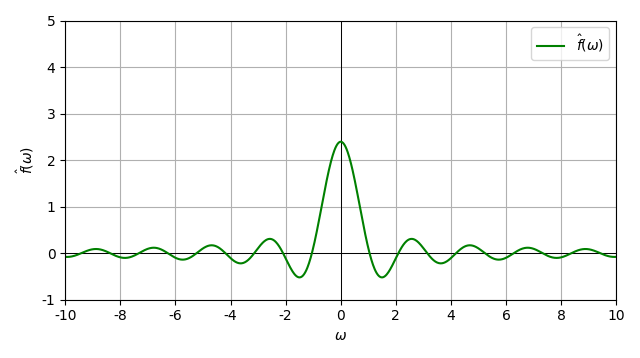
\includegraphics[width=\textwidth]{rectangular/real_fourier_1_3.png}
        \caption{Фурье-образ прямоугольной ф-ии, $a = 1, b = 3$}
    \end{minipage}\\[1em]
        \begin{minipage}{0.5\textwidth}
        \centering 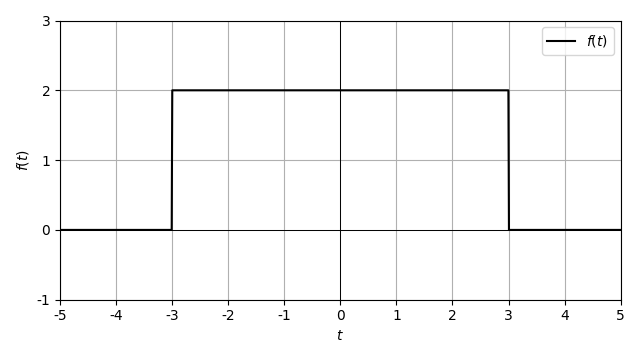
\includegraphics[width=\textwidth]{rectangular/real_graph_2_3.png}
        \caption{Прямоугольная функция, $a = 2, b = 3$}
    \end{minipage}\hfill
    \begin{minipage}{0.5\textwidth}
        \centering 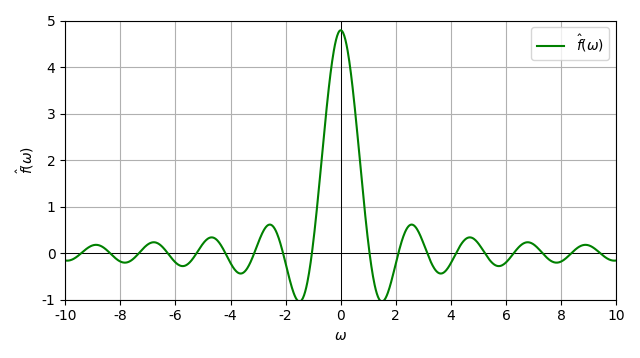
\includegraphics[width=\textwidth]{rectangular/real_fourier_2_3.png}
        \caption{Фурье-образ прямоугольной ф-ии, $a = 2, b = 3$}
    \end{minipage}\\[1em]
\end{figure}\noindent\

По сути, применяя такое преобразование, мы ``растягиваем'' нашу исходную функцию в каждую сторону на $b$ по оси $t$, при этом колебания кардинального синуса становятся плотнее, а амплитуда - больше с увеличением $b$, что является прямым примером свойства растяжения Фурье-оператора. Изменение же параметра $a$ ведёт, во-первых, к повышению ``высоты прямоугольника'' на графике исходной функции, во-вторых, к увеличению амплитуды кардинального синуса на графике Фурье-образа.\

Равенство Парсеваля для преобразования Фурье в общем случае может быть проверено следующим образом:

$$\int_{-\infty}^{\infty}\left\lvert f(t)\right\rvert^2dt = \int_{-\infty}^{\infty}\left\lvert \hat{f}(\omega)\right\rvert^2d\omega$$

\begin{lstlisting}[caption={Равенство Парсеваля при $a = 1, b = 1$}, numbers=none]
| ||f||^2 - ||F||^2 | = 0.0063173
\end{lstlisting}

\begin{lstlisting}[caption={Равенство Парсеваля при $a = 1, b = 3$}, numbers=none]
| ||f||^2 - ||F||^2 | = 0.0063259
\end{lstlisting}

\begin{lstlisting}[caption={Равенство Парсеваля при $a = 2, b = 3$}, numbers=none]
| ||f||^2 - ||F||^2 | = 0.0253036
\end{lstlisting}\ 

Из приведённых расчётов становится понятно, что при увеличении параметра $a$ равенство Парсеваля выполняется хуже.\

\subsection{Треугольная функция}\

Новый подопытный выглядит следующим образом:\

$$
f(t) = \begin{cases}
    a - \left|at/b\right|, & \left| t \right| \leq b \\
    0, & \left| t \right| > b
\end{cases}
$$\

Как и прямоугольная, треугольная функция равна нулю везде кроме маленького отрезка $[-b, b]$, поэтому снова при нахождении Фурье-образа в пределах интегрирования $b$ заменит собой бесконечность:\

$$\hat{f}(\omega)=\frac{1}{\sqrt{2\pi}}\int_{-b}^{b}\left( a - \left| \frac{at}{b} \right| \right)\e^{-i\omega t}dt = \frac{a}{\sqrt{2\pi}}\left( \int_{-b}^{0}\left( 1 + \frac{t}{b} \right)\e^{-i\omega t}dt + \int_{0}^{b}\left( 1 - \frac{t}{b} \right)\e^{-i\omega t}dt \right) = $$
$$= \frac{a}{\sqrt{2\pi}}\left( \int_{-b}^{0}\left( 1 + \frac{t}{b} \right)\e^{-i\omega t}dt + \int_{0}^{b}\left( 1 - \frac{t}{b} \right)\e^{-i\omega t}dt\right) = \frac{a}{\sqrt{2\pi}}\left( \frac{(1 + i\omega (t + b))\e^{-i\omega t}}{b\omega^2}\at^0_{-b} - \frac{(1 + i\omega (t - b))\e^{-i\omega t}}{b\omega^2}\at^b_0 \right) = $$
$$= \frac{a}{\sqrt{2\pi}}\left( \frac{i\omega b + 1 - \e^{i\omega b}}{b\omega^2} - \frac{\e^{-i\omega b} - 1 + i\omega b}{b\omega^2} \right) = \frac{-a}{\omega^2b\sqrt{2\pi}}\left( \e^{-i\omega b} + \e^{i\omega b} - 2 \right) =
$$
$$= \frac{a(2 - 2\cos\omega b)}{\omega^2b\sqrt{2\pi}} = \begin{pmatrix}
    1 - \cos{x} = 2\sin^2\frac{x}{2}\end{pmatrix} = \frac{4a\sin^2{\frac{\omega b}{2}}}{\omega^2 b\sqrt{2\pi}} = \frac{ab}{\sqrt{2\pi}}\mathrm{sinc}^2\,\frac{\omega b}{2}$$

И снова в результате получился кардинальный синус.\ 

Графики для такой функции:

\begin{figure}[H]
    \begin{minipage}{0.5\textwidth}
        \centering 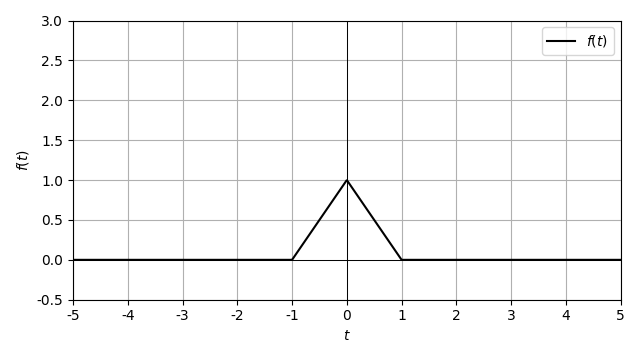
\includegraphics[width=\textwidth]{triangular/real_graph_1_1.png}
        \caption{Треугольная функция, $a = 1, b = 1$}
    \end{minipage}\hfill
    \begin{minipage}{0.5\textwidth}
        \centering 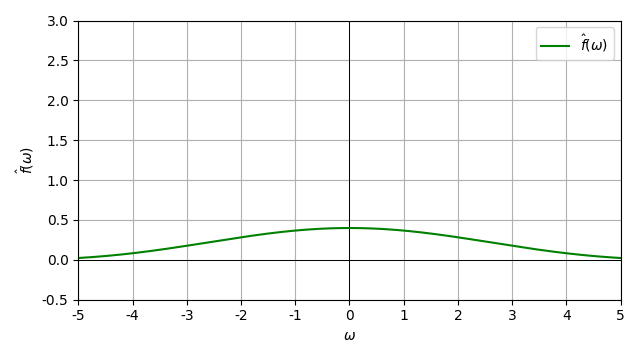
\includegraphics[width=\textwidth]{triangular/real_fourier_1_1.png}
        \caption{Фурье-образ треугольной ф-ии, $a = 1, b = 1$}
    \end{minipage}\\[1em]
        \begin{minipage}{0.5\textwidth}
        \centering 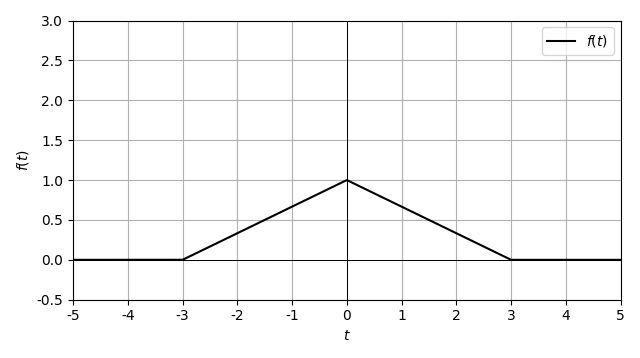
\includegraphics[width=\textwidth]{triangular/real_graph_1_3.png}
        \caption{Треугольная функция, $a = 1, b = 3$}
    \end{minipage}\hfill
    \begin{minipage}{0.5\textwidth}
        \centering 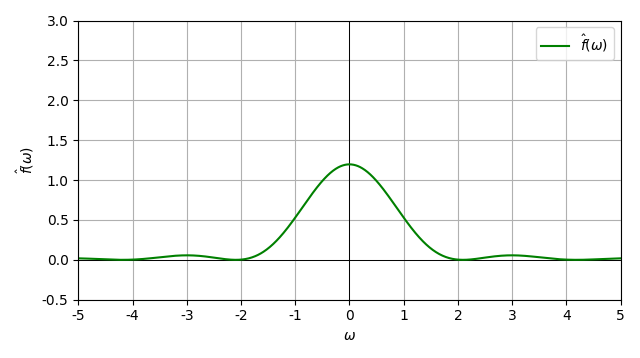
\includegraphics[width=\textwidth]{triangular/real_fourier_1_3.png}
        \caption{Фурье-образ треугольной ф-ии, $a = 1, b = 3$}
    \end{minipage}\\[1em]
\end{figure}\noindent\

\begin{figure}[H]
        \begin{minipage}{0.5\textwidth}
        \centering 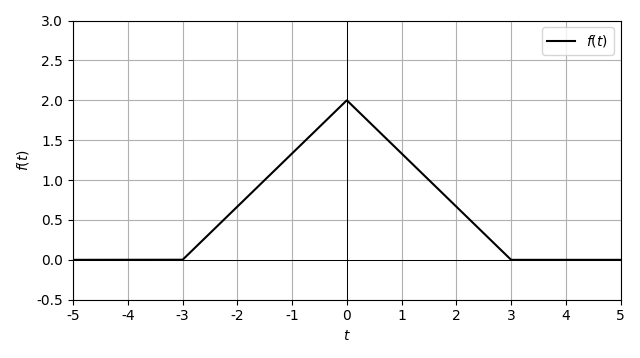
\includegraphics[width=\textwidth]{triangular/real_graph_2_3.png}
        \caption{Треугольная функция, $a = 2, b = 3$}
    \end{minipage}\hfill
    \begin{minipage}{0.5\textwidth}
        \centering 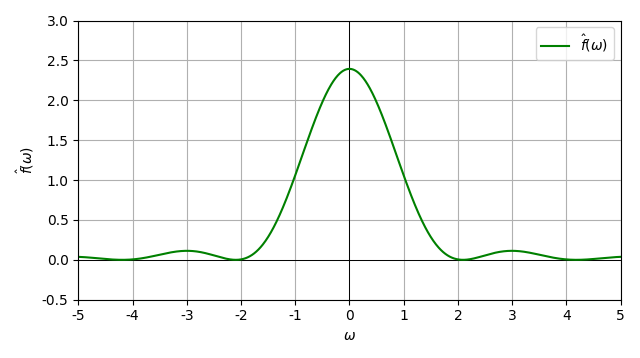
\includegraphics[width=\textwidth]{triangular/real_fourier_2_3.png}
        \caption{Фурье-образ треугольной ф-ии, $a = 2, b = 3$}
    \end{minipage}\\[1em]
\end{figure}\noindent\

Из приведённых графиков становится понятно влияние коэффициентов на внешний вид функции --- параметр $a$ отвечает за высоту треугольника, $b$ - за его ширину. Также можно сделать предположение о влиянии параметров на график Фурье-образа: чем выше треугольник, тем сильнее амплитуда начального колебания (и, соответственно, последующих). Если взглянуть на формулу для $\hat{f}(\omega)$, можно понять, что изменение $a$ влияет на амплитуду кардинального синуса, а изменение $b$ --- и на амплитуду, и на частоту. Это же видно и из графиков.\

Проверим равенство Парсеваля для треугольной функции:

\begin{lstlisting}[caption={Равенство Парсеваля при $a = 1, b = 1$}, numbers=none]
| ||f||^2 - ||F||^2 | = 0.0000006
\end{lstlisting}

\begin{lstlisting}[caption={Равенство Парсеваля при $a = 1, b = 3$}, numbers=none]
| ||f||^2 - ||F||^2 | = 0.0007016
\end{lstlisting}

\begin{lstlisting}[caption={Равенство Парсеваля при $a = 2, b = 3$}, numbers=none]
| ||f||^2 - ||F||^2 | = 0.0028065
\end{lstlisting}\ 

Из приведённых расчётов становится понятно, что с увеличением параметров равенство Парсеваля выполняется хуже.\

\subsection{Кардинальный синус}\

Кардинальный синус $f(t)=a\ sinc(bt)$, получавшийся результатом расчётов Фурье-образов двух последних функций, также может быть представлен через преобразование Фурье. Из готовых таблиц преобразований Фурье зная, что

$$
\int\limits_{-\infty}^\infty \operatorname{sinc}\left(t\right)\,e^{-2\pi i \nu t}dt = \operatorname{rect}\left(\nu\right)\text{, где }\mathrm{rect}(\xi) = \begin{cases}
0,           & |\xi| > \frac{1}{2} \\[3pt]
1,           & |\xi| \leq \frac{1}{2}
\end{cases},
$$\

Для случая с угловой частотой:

$$
\frac{1}{\sqrt{2\pi}} \int\limits_{-\infty}^\infty \operatorname{sinc}\left(t\right)\,\e^{-i\omega t}dt = \frac{1}{\sqrt{2\pi}} \mathrm{rect} \left( \frac{\omega}{2\pi}\right),
$$

Тогда, также помня про свойство растяжения Фурье-оператора $F\{ f(at)\}=\frac{1}{|a|} F\{ f\} \left( \frac{\nu}{a}\right)$:

$$
\hat{f}(\omega) = \frac{1}{\sqrt{2\pi}}\int_{-\infty}^{\infty}a\ \mathrm{sinc}(bt) \e^{-i\omega t}\,dt = \begin{pmatrix}u = bt\end{pmatrix}= \frac{a}{\sqrt{2\pi}|b|}\int_{-\infty}^{\infty}\ \mathrm{sinc}(u) \e^{-i\omega \frac{u}{b}}\, du =\frac{a\pi}{\sqrt{2\pi} |b|} \mathrm{rect}\left(\frac{\omega}{2 b}\right)
$$

В результате получились следующие графики:

\begin{figure}[H]
    \begin{minipage}{0.5\textwidth}
        \centering 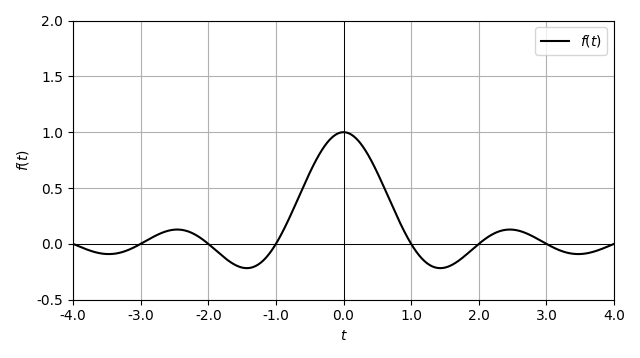
\includegraphics[width=\textwidth]{sinc/real_graph_1_1.png}
        \caption{Кардинальный синус, $a = 1, b = 1$}
    \end{minipage}\hfill
    \begin{minipage}{0.5\textwidth}
        \centering 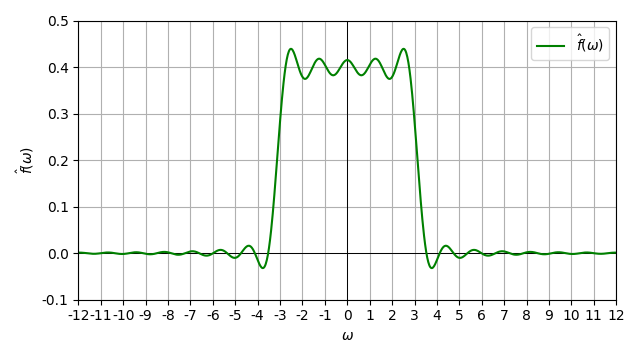
\includegraphics[width=\textwidth]{sinc/real_fourier_1_1.png}
        \caption{Фурье-образ кардинального синуса, $a = 1, b = 1$}
    \end{minipage}\\[1em]
        \begin{minipage}{0.5\textwidth}
        \centering 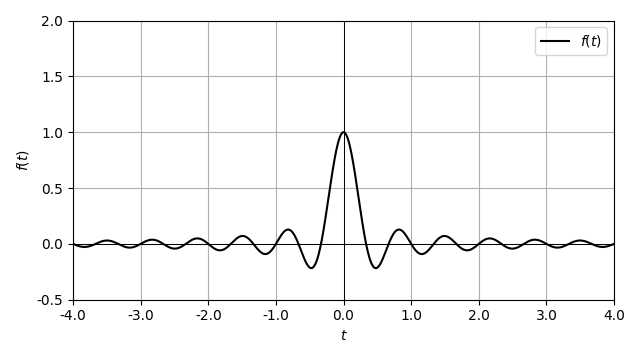
\includegraphics[width=\textwidth]{sinc/real_graph_1_3.png}
        \caption{Кардинальный синус, $a = 1, b = 3$}
    \end{minipage}\hfill
    \begin{minipage}{0.5\textwidth}
        \centering 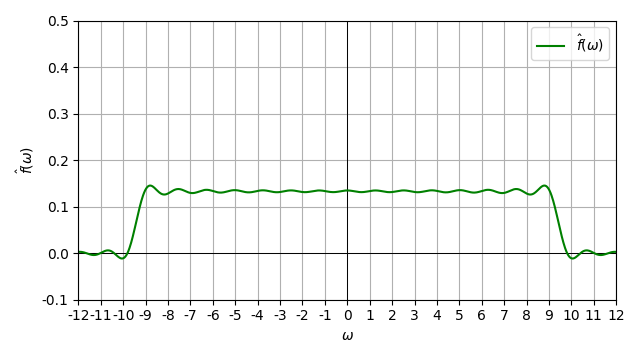
\includegraphics[width=\textwidth]{sinc/real_fourier_1_3.png}
        \caption{Фурье-образ кардинального синуса, $a = 1, b = 3$}
    \end{minipage}\\[1em]
\end{figure}\noindent\
\begin{figure}[H]
        \begin{minipage}{0.5\textwidth}
        \centering 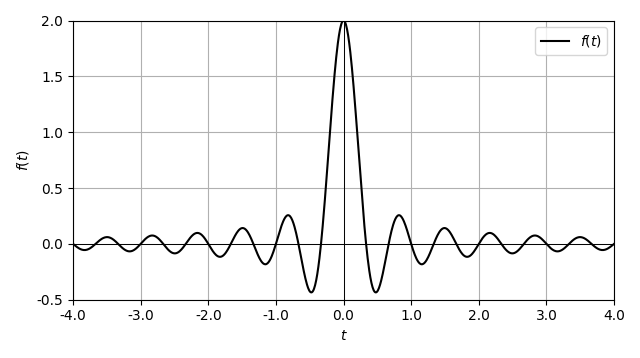
\includegraphics[width=\textwidth]{sinc/real_graph_2_3.png}
        \caption{Кардинальный синус, $a = 2, b = 3$}
    \end{minipage}\hfill
    \begin{minipage}{0.5\textwidth}
        \centering 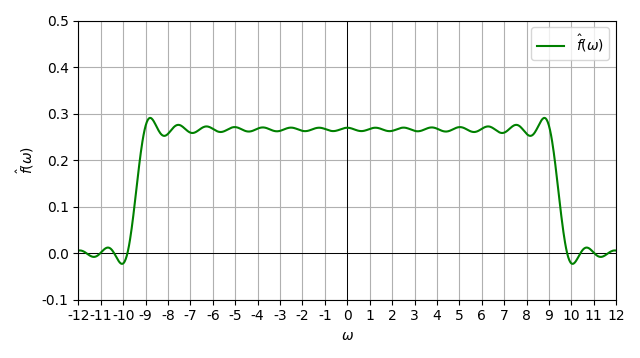
\includegraphics[width=\textwidth]{sinc/real_fourier_2_3.png}
        \caption{Фурье-образ кардинального синуса, $a = 2, b = 3$}
    \end{minipage}\\[1em]
\end{figure}\noindent\

Анализ графиков на предмет влияния изменяемых коэффициентов даёт понять, что $a$ отвечает за начальную амплитуду кардинального синуса, $b$ --- за частоту колебаний, при этом, судя по получившейся формуле для $\hat{f}(\omega)$, параметр $b$ должен снижать амплитуду колебаний Фурье-образа. По графикам Фурье-образов видно, что с увеличением $b$ уменьшается сходимость, колебаний становится заметно больше, и высота графика уменьшается. Немаловажным является то, что в исходной формуле параметр $b$ отвечал за сжатие графика, и, по свойству растяжений, на графике Фурье-образа с увеличением ``сжатости'' графика исходной функции расстояние между соседними колебаниями должно увеличиться, что и отображено на графиках образов.\

Проверим равенство Парсеваля для кардинального синуса:

\begin{lstlisting}[caption={Равенство Парсеваля при $a = 1, b = 1$}, numbers=none]
| ||f||^2 - ||F||^2 | = 0.0000001
\end{lstlisting}

\begin{lstlisting}[caption={Равенство Парсеваля при $a = 1, b = 3$}, numbers=none]
| ||f||^2 - ||F||^2 | = 0.0000001
\end{lstlisting}

\begin{lstlisting}[caption={Равенство Парсеваля при $a = 2, b = 3$}, numbers=none]
| ||f||^2 - ||F||^2 | = 0.0000001
\end{lstlisting}\ 

Из приведённых расчётов становится понятно, что равенство Парсеваля выполняется с довольно высокой точностью, а при малых $a$ и $b$ разница незаметна (ради интереса я даже взял коэффициенты равными $10$ и $30$, отклонение стало равным $0.0000650$).\

\subsection{Функция Гаусса}\

В этот раз на рассмотрении находится следующая функция:
$$
f(t) = a\e^{-bt^2}
$$

Фурье преобразование в этом случае будет следующим:

$$
\frac{1}{\sqrt{2\pi}} \int_{-\infty}^{\infty} a\ \e^{-bt^2}\ \e^{-i\omega t}\, dt = 
\frac{a}{\sqrt{2\pi}} \int_{-\infty}^{\infty} \e^{-bt^2 - i \omega t} dt
$$\ 

Это --- Гауссов интеграл вида $\int_{-\infty}^{\infty} e^{At^2+Bt}\, dt=\sqrt{\frac{\pi}{A}}e^{\frac{B^2}{4A}}$, в котором $A = -b, B = -i\omega$. Подставим значения в формулу и получим следующее:

$$
\hat{f}(\omega) = \frac{a}{\sqrt{2\pi}}\cdot\sqrt{\frac{\pi}{b}}\e^{-\frac{\omega^2}{4b}}=\frac{a}{\sqrt{2b}}\e^{-\frac{\omega^2}{4b}}
$$

Визуализация графика функции Гаусса и её Фурье-образа:

\begin{figure}[H]
    \begin{minipage}{0.5\textwidth}
        \centering 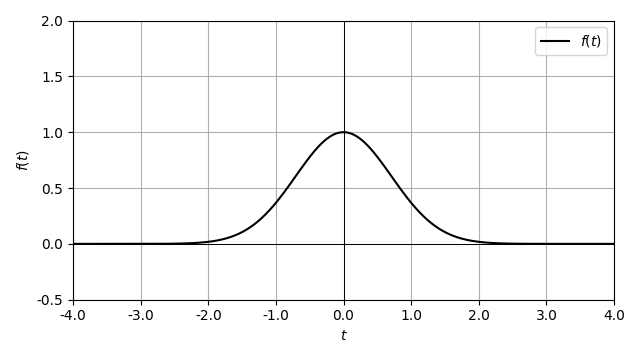
\includegraphics[width=\textwidth]{gaussian/real_graph_1_1.png}
        \caption{Функция Гаусса, $a = 1, b = 1$}
    \end{minipage}\hfill
    \begin{minipage}{0.5\textwidth}
        \centering 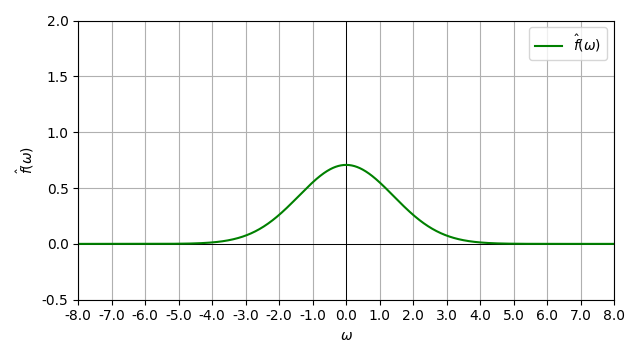
\includegraphics[width=\textwidth]{gaussian/real_fourier_1_1.png}
        \caption{Фурье-образ функции Гаусса, $a = 1, b = 1$}
    \end{minipage}\\[1em]
\end{figure}\noindent\
\begin{figure}[H]
        \begin{minipage}{0.5\textwidth}
        \centering 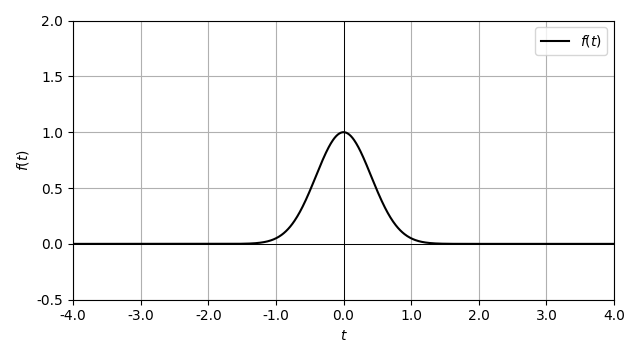
\includegraphics[width=\textwidth]{gaussian/real_graph_1_3.png}
        \caption{Функция Гаусса, $a = 1, b = 3$}
    \end{minipage}\hfill
    \begin{minipage}{0.5\textwidth}
        \centering 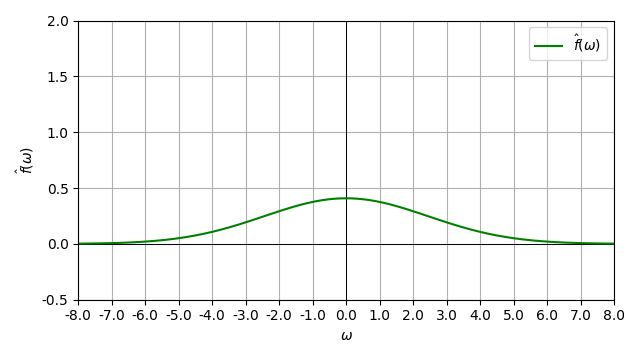
\includegraphics[width=\textwidth]{gaussian/real_fourier_1_3.png}
        \caption{Фурье-образ функции Гаусса, $a = 1, b = 3$}
    \end{minipage}\\[1em]
        \begin{minipage}{0.5\textwidth}
        \centering 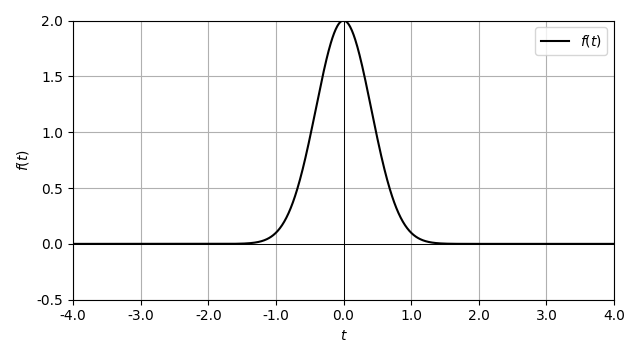
\includegraphics[width=\textwidth]{gaussian/real_graph_2_3.png}
        \caption{Функция Гаусса, $a = 2, b = 3$}
    \end{minipage}\hfill
    \begin{minipage}{0.5\textwidth}
        \centering 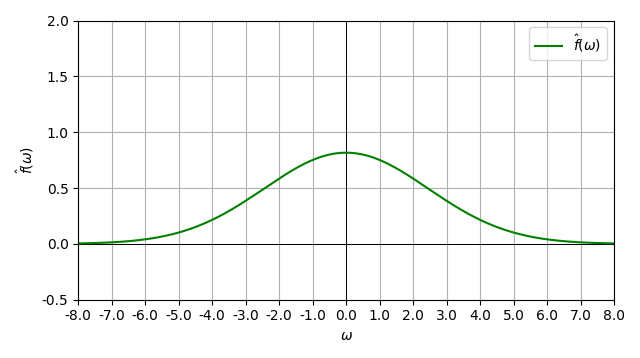
\includegraphics[width=\textwidth]{gaussian/real_fourier_2_3.png}
        \caption{Фурье-образ функции Гаусса, $a = 2, b = 3$}
    \end{minipage}\\[1em]
\end{figure}\noindent\

По данным графикам можно однозначно утверждать, что $a$ отвечает за ``высоту'' функции в начальный момент времени (амплитуду), а $b$ --- за ``ширину'', влияя при этом в обратную сторону. На Фурье-образ влияние же аналогичное, но теперь увеличение $b$ прямо пропорционально увеличению ``ширины'' функции (скорости убывания функции) и к тому же влияет на значение функции при $\omega=0$ (чем меньше $b$, тем больше $\hat{f}(\omega)$). С точки зрения свойств преобразования Фурье, выполняется линейность --- $f(t)$ умножена на $a$, и $\hat{f}(\omega)$ увеличилась в $a$ раз.\

Проверим равенство Парсеваля для функции Гаусса:

$$\left\lVert f \right\rVert _2 = \left\lVert \mathcal{F} \right\rVert _2 \quad\Rightarrow\quad \int_{-\infty}^{\infty}\left\lvert f(t)\right\rvert^2dt = \int_{-\infty}^{\infty}\left\lvert \hat{f}(\omega)\right\rvert^2d\omega$$

\begin{lstlisting}[caption={Равенство Парсеваля при $a = 1, b = 1$}, numbers=none]
| ||f||^2 - ||F||^2 | = 0.0000021
\end{lstlisting}

\begin{lstlisting}[caption={Равенство Парсеваля при $a = 1, b = 3$}, numbers=none]
| ||f||^2 - ||F||^2 | = 0.0000000
\end{lstlisting}

\begin{lstlisting}[caption={Равенство Парсеваля при $a = 2, b = 3$}, numbers=none]
| ||f||^2 - ||F||^2 | = 0.0000000
\end{lstlisting}\ 

Как итог проверки равенства Парсеваля можно сказать, что оно выполняется в некотором приближении при всех рассмотренных коэффициентах, и немного лучше выполняется при $b = 3$.

\subsection{Двустороннее затухание}\

Последняя функция в вещественном задании --- $f(t) = a \e^{-b|t|}$.\

Фурье преобразование для неё следующее:\

$$
\hat{f}(\omega) = \frac{1}{\sqrt{2\pi}}\int_{-\infty}^{\infty} a \e^{-b|t|} \e^{-i\omega t}\,dt = \frac{a}{\sqrt{2\pi}} \int_{-\infty}^{\infty} \e^{-b|t| -i\omega t}\,dt = \frac{a}{\sqrt{2\pi}} \left(\int_{-\infty}^{0} \e^{(b -i\omega)t} + \int_{0}^{\infty} \e^{-(b +i\omega)t}\right)
$$
$$
= \frac{a}{\sqrt{2\pi}}\left( \frac{\e^{t(b-i\omega)}}{b - i\omega}\at^0_{-\infty} + \frac{\e^{-t(b + i\omega)}}{b + i\omega}\at^0_\infty \right) = \frac{a}{\sqrt{2\pi}}\left( \frac{1}{b - i\omega} - \frac{0}{b - i\omega} + \frac{1}{b+i\omega} - \frac{0}{b+i\omega} \right) =
$$
$$
= \frac{a}{\sqrt{2\pi}}\left( \frac{1}{b-i\omega} + \frac{1}{b+i\omega} \right) = \frac{2ab}{\sqrt{2\pi}(b^2 + \omega^2)} = \frac{ab}{(b^2+\omega^2)}\sqrt{\frac{2}{\pi}}
$$

Визуализация этой функции:

\begin{figure}[H]
    \begin{minipage}{0.5\textwidth}
        \centering 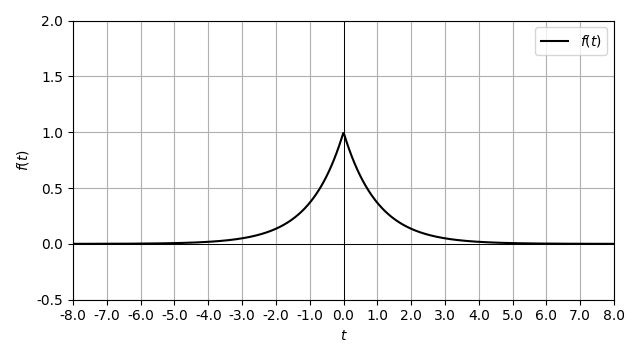
\includegraphics[width=\textwidth]{fade/real_graph_1_1.png}
        \caption{Двустороннее затухание, $a = 1, b = 1$}
    \end{minipage}\hfill
    \begin{minipage}{0.5\textwidth}
        \centering 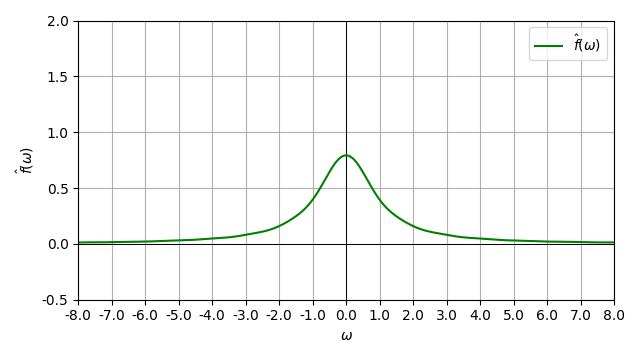
\includegraphics[width=\textwidth]{fade/real_fourier_1_1.png}
        \caption{Фурье-образ двустороннего затухания, $a = 1, b = 1$}
    \end{minipage}\\[1em]
        \begin{minipage}{0.5\textwidth}
        \centering 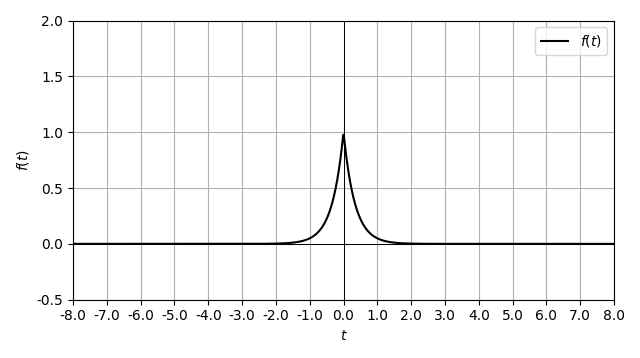
\includegraphics[width=\textwidth]{fade/real_graph_1_3.png}
        \caption{Двустороннее затухание, $a = 1, b = 3$}
    \end{minipage}\hfill
    \begin{minipage}{0.5\textwidth}
        \centering 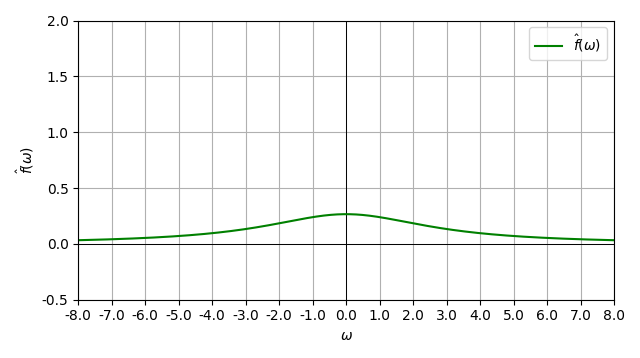
\includegraphics[width=\textwidth]{fade/real_fourier_1_3.png}
        \caption{Фурье-образ двустороннего затухания, $a = 1, b = 3$}
    \end{minipage}\\[1em]
\end{figure}\noindent\
\begin{figure}[H]
        \begin{minipage}{0.5\textwidth}
        \centering 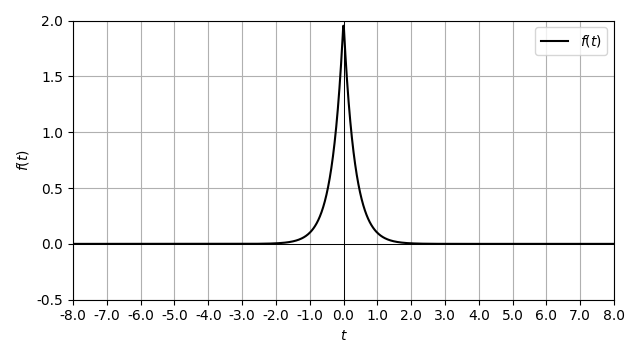
\includegraphics[width=\textwidth]{fade/real_graph_2_3.png}
        \caption{Двустороннее затухание, $a = 2, b = 3$}
    \end{minipage}\hfill
    \begin{minipage}{0.5\textwidth}
        \centering 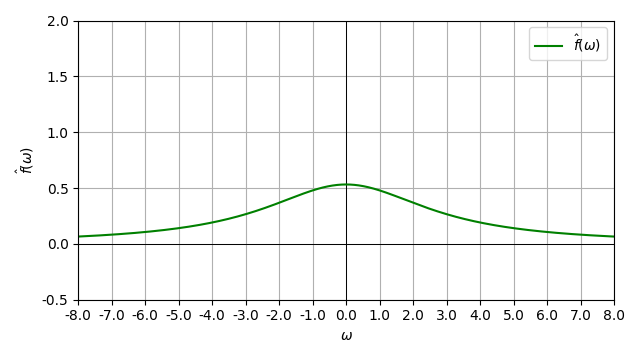
\includegraphics[width=\textwidth]{fade/real_fourier_2_3.png}
        \caption{Фурье-образ двустороннего затухания, $a = 2, b = 3$}
    \end{minipage}\\[1em]
\end{figure}\noindent\

Снова на лицо выполнение свойства линейности. В исходной функции $b$ влияет на ширину основания треугольника (если это можно так назвать), а $a$ --- на длину его высоты. И, согласно формуле Фурье-образа, с изменением $a$ изменяется амплитуда кардинального синуса, а изменение $b$ приводит к изменению не только амплитуды, но и частоты (на графике это становится особенно заметно, если взять $b=0.5$)\

Проверим равенство Парсеваля для двустороннего затухания:

$$\left\lVert f \right\rVert _2 = \left\lVert \mathcal{F} \right\rVert _2 \quad\Rightarrow\quad \int_{-\infty}^{\infty}\left\lvert f(t)\right\rvert^2dt = \int_{-\infty}^{\infty}\left\lvert \hat{f}(\omega)\right\rvert^2d\omega$$

\begin{lstlisting}[caption={Равенство Парсеваля при $a = 1, b = 1$}, numbers=none]
| ||f||^2 - ||F||^2 | = 0.0000021
\end{lstlisting}

\begin{lstlisting}[caption={Равенство Парсеваля при $a = 1, b = 3$}, numbers=none]
| ||f||^2 - ||F||^2 | = 0.0000038
\end{lstlisting}

\begin{lstlisting}[caption={Равенство Парсеваля при $a = 2, b = 3$}, numbers=none]
| ||f||^2 - ||F||^2 | = 0.0000153
\end{lstlisting}\ 

В этом случае увеличение коэффициентов негативно сказывается на выполнении равенства Парсеваля.

\subsection{Выводы по вещественному}\

Как итог, хочется отметить выполнение свойств преобразования Фурье и неплохую точность равенства Парсеваля.

\section{Комплексное задание}

Сдвигать я решил функцию двустороннего затухания, с $a$ и $b$ соответственно равными $2$ и $3$. Вот как она будет выглядеть:

$$
f(t) = 2\e^{-3|t|}
$$

Рассматривая $g(t) = f(t + c) = 2\e^{-3|t+c|}$ в общем случае, можно получить аналитическое выражение Фурье-образа $\hat{g}(\omega)$:

$$
\hat{g}(\omega) = \int_{-\infty}^\infty 2\e^{-3|t+c|} \, \e^{-i\omega t}\, dt = 
\e^{i\omega c}\hat{f}(\omega) = \frac{6\e^{i\omega c}}{(9+\omega^2)}\sqrt{\frac{2}{\pi}}
$$\

Переход $\hat{g}(\omega)=\e^{i\omega c}\hat{f}(\omega)$ обусловлен свойством сдвига, рассмотренным на лекции 3, а $\hat{g}(\omega)$ было взято из пункта 1.5.

При построении графиков $g(t)$ использованы значения параметра из списка $[1, 2, -1]$. 
\begin{figure}[H]
        \centering 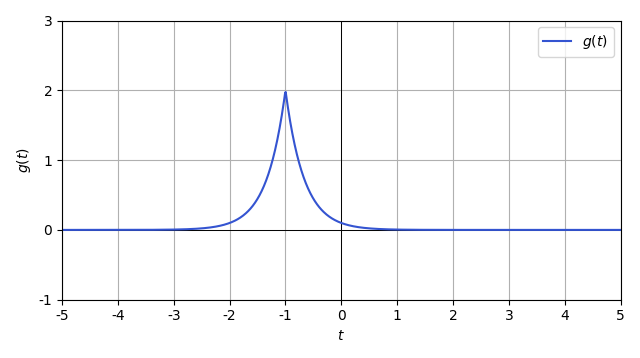
\includegraphics[width=\textwidth]{complex/graph_default/complex_graph_2_3_-1.png}
        \caption{$g(t) = f(t-1)$}
\end{figure}\noindent\
\begin{figure}[H]
        \centering 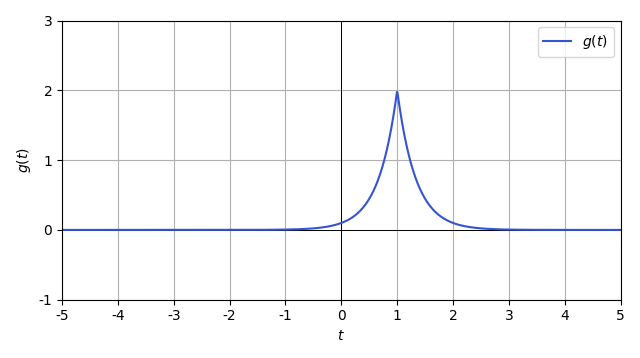
\includegraphics[width=\textwidth]{complex/graph_default/complex_graph_2_3_1.png}
        \caption{$g(t) = f(t+1)$}
\end{figure}\noindent\
\begin{figure}[H]
        \centering 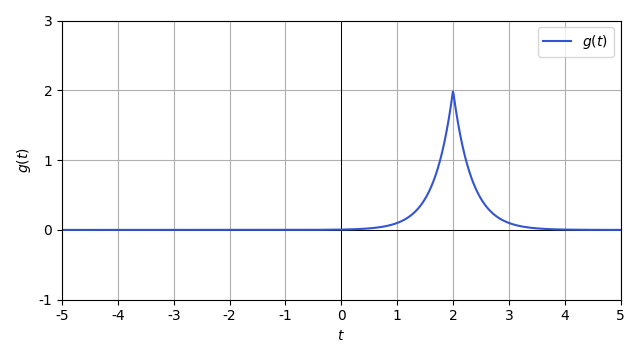
\includegraphics[width=\textwidth]{complex/graph_default/complex_graph_2_3_2.png}
        \caption{$g(t) = f(t+2)$}
\end{figure}\noindent\

Из графиков видно, что, как и ожидалось, изменение параметра $c$ приводит к смещению функции по оси $t$.

\begin{figure}[H]
        \centering 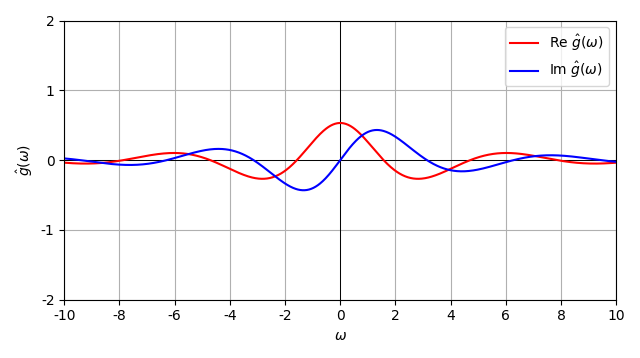
\includegraphics[width=\textwidth]{complex/complex_fourier_2_3_-1.png}
        \caption{Фурье-образ при $c = -1$}
\end{figure}\noindent\
\begin{figure}[H]
        \centering 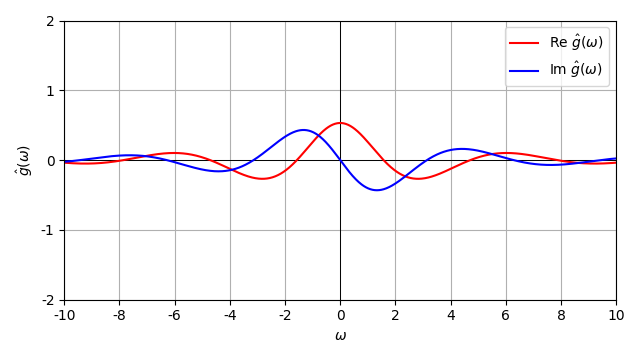
\includegraphics[width=\textwidth]{complex/complex_fourier_2_3_1.png}
        \caption{Фурье-образ при $c = 1$}
\end{figure}\noindent\
\begin{figure}[H]
        \centering 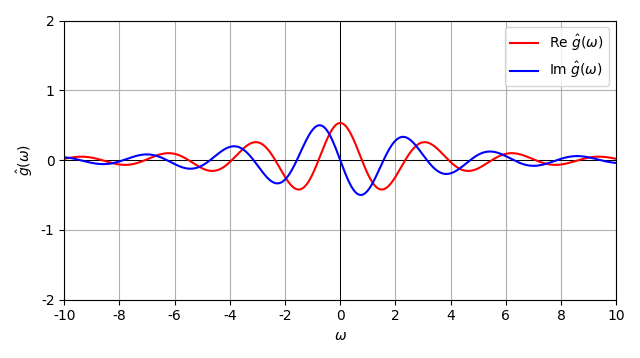
\includegraphics[width=\textwidth]{complex/complex_fourier_2_3_2.png}
        \caption{Фурье-образ при $c = 2$}
\end{figure}\noindent\

Заметно, что вещественная часть Фурье-образов совпадает при $c=1$ и $c=-1$, при этом мнимая часть отражается относительно оси ординат при смене знака коэффициента, что и понятно.

\begin{figure}[H]
        \centering 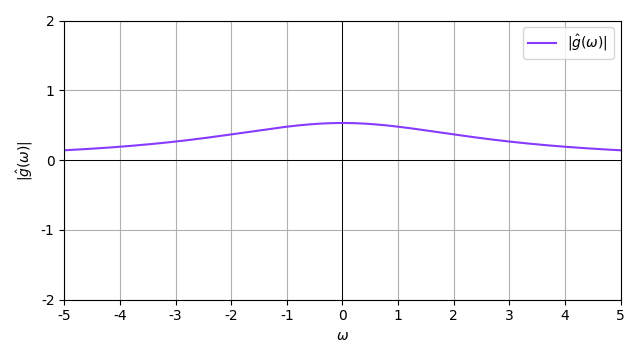
\includegraphics[width=\textwidth]{complex/complex_abs_2_3_-1.png}
        \caption{$|\hat{g}(\omega)|$ при $c = -1$}
\end{figure}\noindent\
\begin{figure}[H]
        \centering 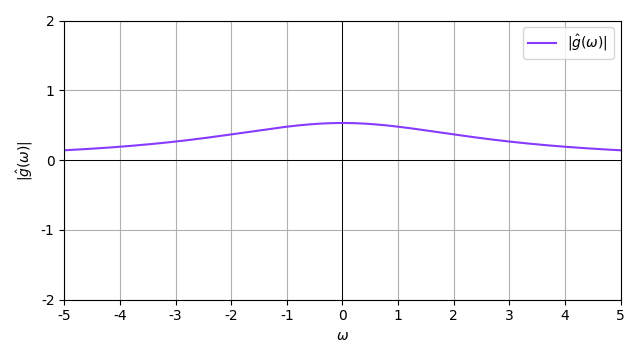
\includegraphics[width=\textwidth]{complex/complex_abs_2_3_1.png}
        \caption{$|\hat{g}(\omega)|$ при $c = 1$}
\end{figure}\noindent\
\begin{figure}[H]
        \centering 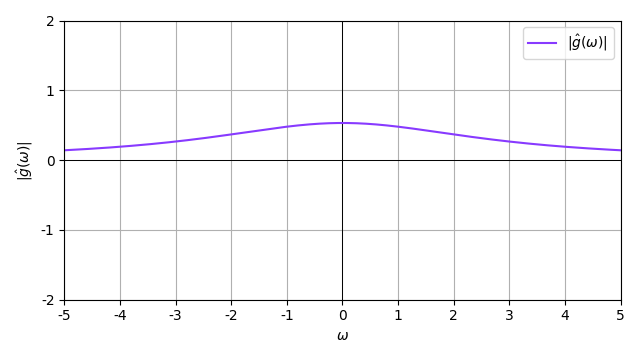
\includegraphics[width=\textwidth]{complex/complex_abs_2_3_2.png}
        \caption{$|\hat{g}(\omega)|$ при $c = 2$}
\end{figure}\noindent\

При небольших сдвигах исходной функции модуль Фурье-образа остаётся почти неизменным, это объясняется тем, что по определению модуль Фурье-образа сдвинутой функции это модуль Фурье-функции исходной функции, умноженной на модуль мнимой экспоненты. Поскольку последний всегда равен единице, модуль Фурье-образа сдвинутой функции остается неизменным, меняется только его фаза.

\subsubsection*{Выводы по комплексному}\

В результате выполнения этого задания я убедился в том, что свойство сдвига Фурье-образа выполняется (сначала посчитал без него руками), а также стал более естественно воспринимать преобразование Фурье.

\section{Музыкальное задание}\

В последнем задании будет использовано преобразование Фурье к обычной частоте $\nu$:

$$\hat{f}(\nu) = \int_{-\infty}^{\infty}f(t)\e^{-2\pi i\nu t}\,dt$$\

Аккорд я взял под номером 25. Код $Matlab$ для поиска Фурье-образа аккорда при помощи численного интегрирования получился следующим:

\begin{lstlisting}[language=Matlab, caption={Нахождение Фурье-образа $\hat{f}(\nu)$}]
    [audio, fs] = audioread('Аккорд (25).mp3');
    
    if size(audio, 2) > 1
        audio = audio(:, 1); 
    end
    
    N = length(audio);
    t = (0:N-1) / fs;
    t = t(:);
    
    V = 1000;  % Максимальная частота анализа
    dv = 1;    % Шаг по частоте
    v = (0:dv:V)';  % Вектор частот (столбец)
    Y = zeros(size(v)); % Выделяем память
    
    for k = 1:length(v)
        exp_term = exp(-1i * 2 * pi * v(k) * t);
        Y(k) = trapz(t, audio .* exp_term); % Преобразование Фурье
    end
\end{lstlisting}\

Построение графиков $f(t)$ и $|\hat{f}(\nu)|$ также выполнено в $Matlab$:

\begin{figure}[H]
    \begin{minipage}{0.5\textwidth}
        \centering \includegraphics[width=\textwidth]{music/|f(omega)|.png}
        \caption{$|\hat{f}(\nu)|$}
    \end{minipage}
    \begin{minipage}{0.5\textwidth}
        \centering 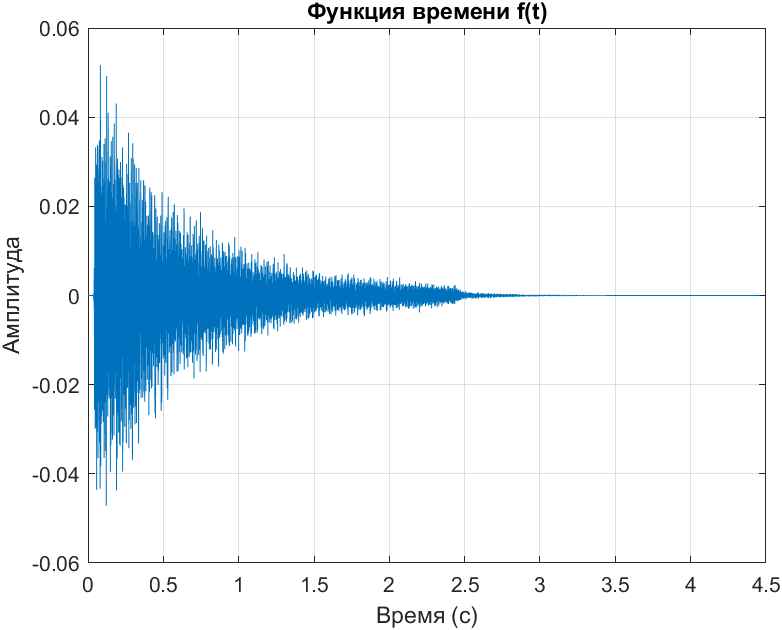
\includegraphics[width=\textwidth]{music/f(t).png}
        \caption{$f(t)$}
    \end{minipage}
\end{figure}\noindent\

По графику модуля Фурье-образа можно заметить пики на некоторых частотах, наибольшие из них на $98, 196, 220, 247, 294, 392, 494, 587, 660$. По \href{https://muted.io/note-frequencies/}{таблице соответствия нот и частот} можно сделать вывод о том, что аккорд составлен из нот G2, G3, A3, B3, D4, E4, B4, D5, E5. На самом деле не совсем понятно, какой минимальный модуль Фурье-образа считается за ноту, ведь можно взять частоты, модуль образа которых не превышает $0.05$, но тогда появляется вероятность учесть частоты от сторонних шумов.
\subsection{Выводы по музыкальному}\

В результате выполнения задания я осознал, насколько преобразование Фурье прикладное, также обдумал другие варианты его использования --- ведь не только звук можно раскладывать на частоты, наверняка также можно поступить и с визуальной информацией, найдя для этого уйму применений.

\section{Общие выводы}\

При выполнении работы я наглядно убедился в том, что свойства Фурье-преобразования работают, открыл для себя новое, чего не запомнил из лекционного материала (к примеру, неизменность модуля Фурье-образа при сдвиге исходной функции), проанализировал реальный сигнал и посмотрел на особенности спектральных представлений различных функций (Фурье-образ прямоугольной функции --- кардинальный синус, а Фурье-образ кардинального синуса --- прямоугольная функция).

\end{document}